
\documentclass[paper=a4, fontsize=11pt]{scrartcl} % A4 paper and 11pt font size

\usepackage[T1]{fontenc} % Use 8-bit encoding that has 256 glyphs
\usepackage{fourier} % Use the Adobe Utopia font for the document - comment 
\usepackage[english]{babel} % English language/hyphenation
\usepackage{amsmath,amsfonts,amsthm} % Math packages
\usepackage{graphicx}
\usepackage{float}
\usepackage{subfig}
\usepackage{caption}
\usepackage[section]{placeins}
\usepackage{sectsty} % Allows customizing section commands
\allsectionsfont{\centering \normalfont\scshape} 
\numberwithin{equation}{section} 
\numberwithin{figure}{section} 
\numberwithin{table}{section} 

\setlength\parindent{2pt} 
%-------------------------------------------------------------------------------
%	TITLE SECTION
%-------------------------------------------------------------------------------

\newcommand{\horrule}[1]{\rule{\linewidth}{#1}} % Create horizontal rule command with 1 argument of height

\title{	
\normalfont \normalsize 
\textsc{PH 481 Lab} \\ [25pt] 
\horrule{2pt} \\[0.5cm] % Thin top horizontal rule
\huge Optics Lab 6\\ % The assignment title
\horrule{2pt} \\[0.5cm] % Thick bottom horizontal rule
}

\author{Harsukh Singh} % Your name

\date{\normalsize \today} % Today's date or a custom date

\begin{document}

\maketitle % Print the title
\section{Overview of Experiment}
In this lab we explored Fraunhofer diffraction with both a circular aperature 
and rectangular aperature and we also looked at Fresnel diffraction with circular aperature.  The first part of th lab 
involved building a beam expander using a -25 mm focal length lens followed by a 
100 mm focal length lens, this is labeled as the telescope in the figure below. After this was done we used the usb camera to find the pixel per cm. This was done by imaging a ruler on the usb camer and dividing the number of pixels over the range imaged. We then used the lens equation to find ratio of cm per pixel. This was approximately found to be $6.72 \times 10^{-4} \frac{cm}{pixel}$

\begin{figure}[H]
	\caption{Finding the pixel per cm}
		\begin{center}
			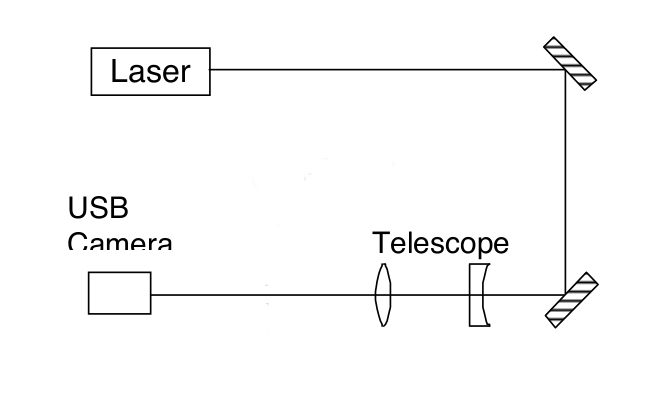
\includegraphics[scale=0.3]{stage}
		\end{center}
\end{figure}
\section{Fraunhofer Diffraction with Circular and Rectangular Aperatures}
The experimental setup is shown below for this is shown in figure 2.1. 
\begin{figure}[H]
\caption{Experimental Set Up}
\begin{center}
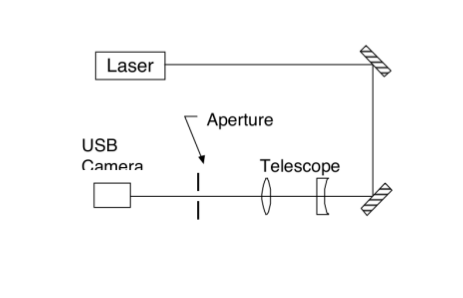
\includegraphics[scale=0.5]{diff}
\end{center}
\end{figure}
\subsection{Rectangular Aperature}
We used the rectangular aperature to find the intensity profile and this is plotted with respect to the distance (cm), shown below,
\begin{figure}[H]
\centering
\parbox{5cm}{
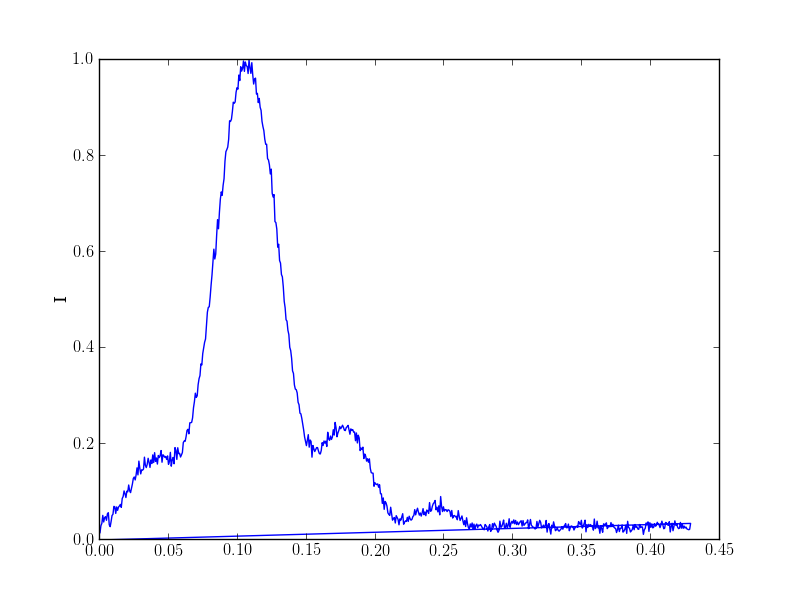
\includegraphics[width=5cm]{rec1}
\caption{Intensity Profile 1}}
\qquad
\begin{minipage}{5cm}
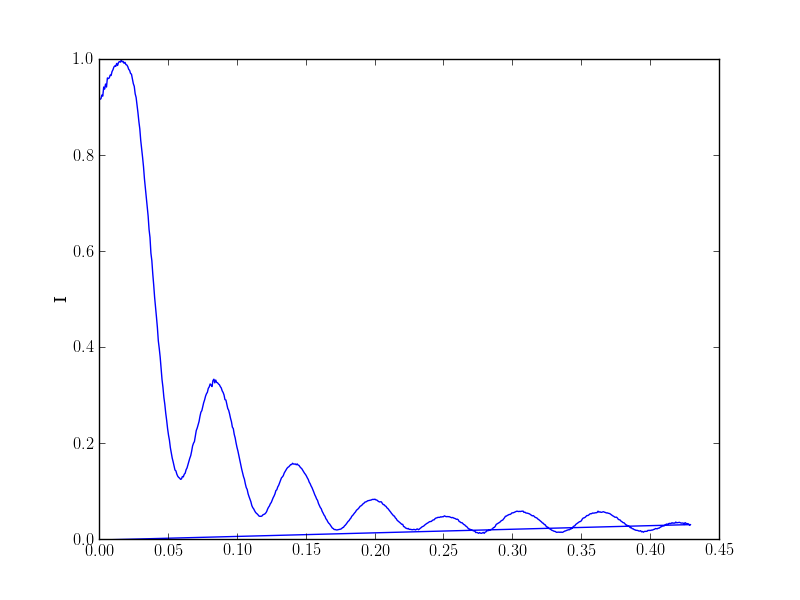
\includegraphics[width=5cm]{rec2}
\caption{Intensity Profile 2}
\end{minipage}
\end{figure}
The size of the aperature can be found using the transverse intensity along the $\beta$ axis as explained in Hecth page pg. 466. We then use the formula 10.44 in Hecht and set it to the first minimum. R was found to be 60 cm and Y was the domain. 
\begin{equation}
b = \frac{2R\pi}{kY}
\end{equation}
The diameter of the aperature was found to be 0.8 mm.
\subsection{Circular Aperature}
With the circular aperature we found the intensity profile shown below,
\begin{figure}[H]
\caption{Circular Aperature Fraunhofer Diffraction}
\begin{center}
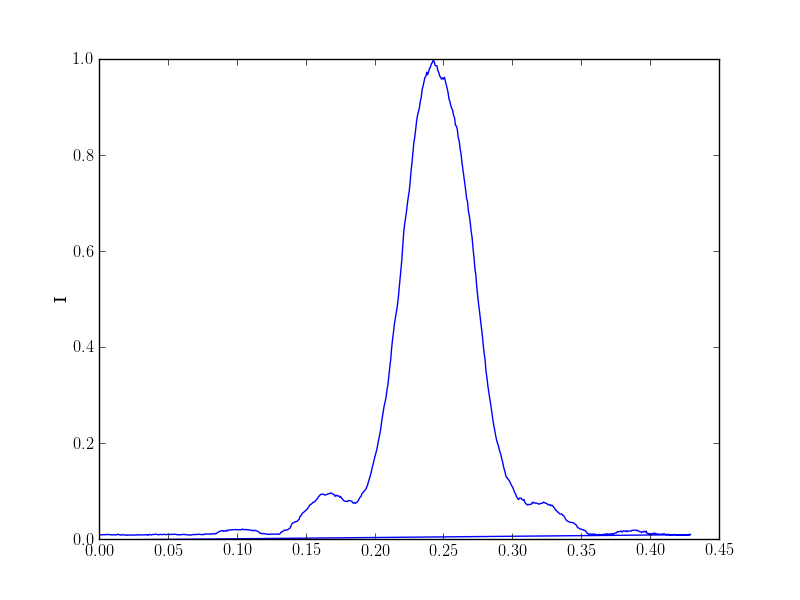
\includegraphics[scale=0.3]{circ}
\end{center}
\end{figure}
We use the equation given in Hecht(10.57).
\begin{equation}
a = 1.22\frac{R\lambda}{2q_1}
\end{equation}
from the graph we find $q_1$ to be, 0.36 cm. So we find the aperature size to be, 0.1 mm.
\section{Fresnel Diffraction with Circular Aperature}
In the case of fresnel diffraction with circular aperature. We moved the 100 mm focal length glass over a varying distance and observed the pattern shown on pg.493 in Hecht thus we were able to create a table below, showing these values.
\begin{table}[H]
  \centering 
   \caption{zones in a circular aperature}
  \begin{tabular}{|l |r| }
    \hline
     m & x(cm) \\ \hline
     1 & 32.9 \\ \hline
     2 & 21.15 \\ \hline
     3 & 16.75 \\ \hline
     4 & 13.85  \\ \hline
     5 & 11.65 \\  \hline
  \end{tabular}
 \end{table}
We then plot the position vs $\frac{1}{n}$ and the plot is shown in figure 3.1.
\begin{figure}[H]
\caption{Position of Minima}
\begin{center}
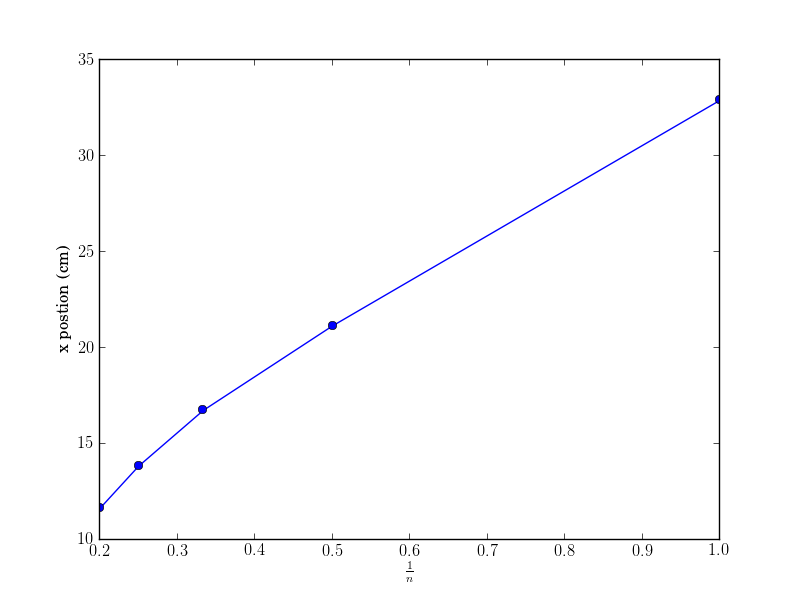
\includegraphics[scale=0.3]{circf}
\end{center}
\end{figure}
from this we fit the data, to the equation $x_n = \frac{R^2}{2n\lambda}$ and find the aperature size to be 0.23 mm.
\section{Conclusion}
There was quite a bit of uncertainty related counting the minima for the fresnel diffraction experiment because as the magnifying lens got closer to the aperature the distance between each zone became closer. So the aperature size was determined smaller region with more data.
\end{document}

%\begin{figure}[htb]
%\centering
%\parbox{5cm}{
%\includegraphics[width=5cm]{figure_1}
%\caption{ Reflection Coefficients}}
%\qquad
%\begin{minipage}{5cm}
%\includegraphics[width=5cm]{figure_2}
%\caption{Transmission Coefficients}
%\end{minipage}
%\end{figure}
%
%\begin{figure}[htb]
%\centering
%\parbox{5cm}{
%\includegraphics[width=5cm]{Epar}
%\caption{Electric Field Parallel to Incident Plane}
%\label{fig:2figsA}}
%\qquad
%\begin{minipage}{5cm}
%\includegraphics[width=5cm]{Eperp}
%\caption{Electric Field Perpendicular to Indicent Plane}
%\label{fig:2figsB}
%\end{minipage}
%%\end{figure}
%
%\section{Experiment 1.1:  Transmittance through Glass}
%\begin{figure}[!ht]
%	\caption{Experimental Set-Up}
%		\begin{center}
%			\includegraphics[scale=0.5]{transmittance}
%		\end{center}
%\end{figure}

%\begin{figure}[!ht]
%	\caption{Experimental Comparison to Theoretical Transmission 
%Coefficients}
%		\begin{center}
%			\includegraphics[scale=0.5]{figure_3}
%		\end{center}
%\end{figure}
%
%\section{Experiment 1.2:  Reflectance from Frosted Glass}
%\begin{figure}[!ht]
%		\begin{center}
%			\includegraphics[scale=0.5]{reflectance}
%		\end{center}
%\caption{Reflectance from Frosted Glass}
%\end{figure}

%\section{Experiment 1.3: Refraction through glass slab}
%\begin{figure}[!ht]
%		\begin{center}
%			\includegraphics[scale=0.5]{GlassLab}
%		\end{center}
%\caption{Measuring the index of refraction through Glass Slab}
%\end{figure}g
% \begin{equation}
%sin(\theta_i -\theta_t) = \frac{l}{\frac{t}{cos(\theta_t)}}
% \end{equation}
% and,
% \begin{equation}
%n_{slab}  = 
%\frac{n_1sin(\theta_1)}{sin(\theta_1-sin^{-1}(\frac{t}{\frac{l}{sin(\theta_i 
%-\theta_t)}}))}
% \end{equation}
% Solving this $n_{slab} = 1.42$  and since most glass has a refractive index 
% of ~1.5 this was pretty close.
% \begin{equation}
%   \begin{tabular}{|l |r| }
%     \hline
%      d(m) & 0.0065561             \\ \hline
%     d^{'} (m) & 0.0064660        \\ \hline
%     d^{''}(m) & 0.006345             \\  \hline
%     d^{'''}(m)& 0.0061452               \\  \hline
%   \end{tabular}
% \end{equation}
% \begin{figure}[htb]
% 	\caption{Fabry-Perot fringes (I vs delta)}
% 		\begin{center}
% 			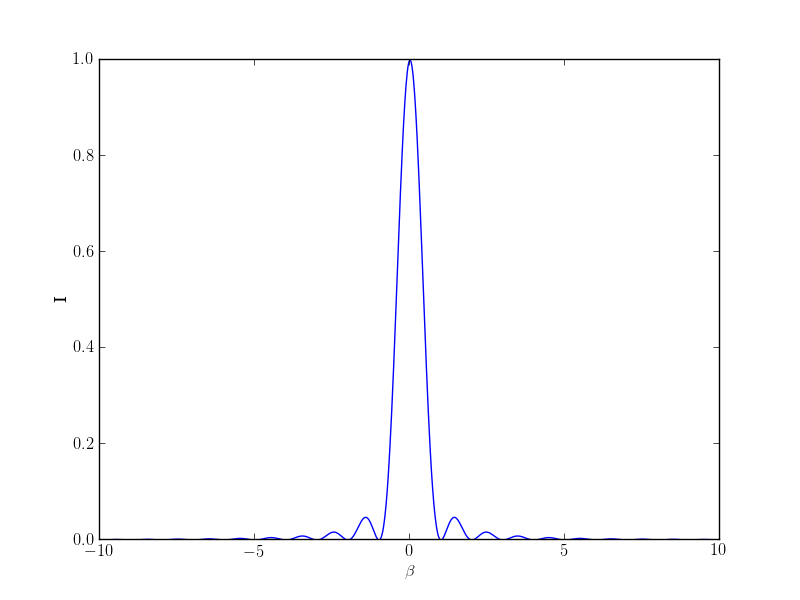
\includegraphics[scale=0.5]{fringes}
% 		\end{center}
% \end{figure}
% \begin{table}[H]
%   \centering 
%    \caption{data}
%   \begin{tabular}{|l |r| }
%     \hline
%      3 slits & $\frac{2}{3}$ \\ \hline
%      4 slits & $\frac{2}{4}$ \\ \hline
%      10 slits & $\frac{2}{3}$ \\  \hline
%   \end{tabular}
% \end{table}
% \begin{figure}[H]
% \centering
% 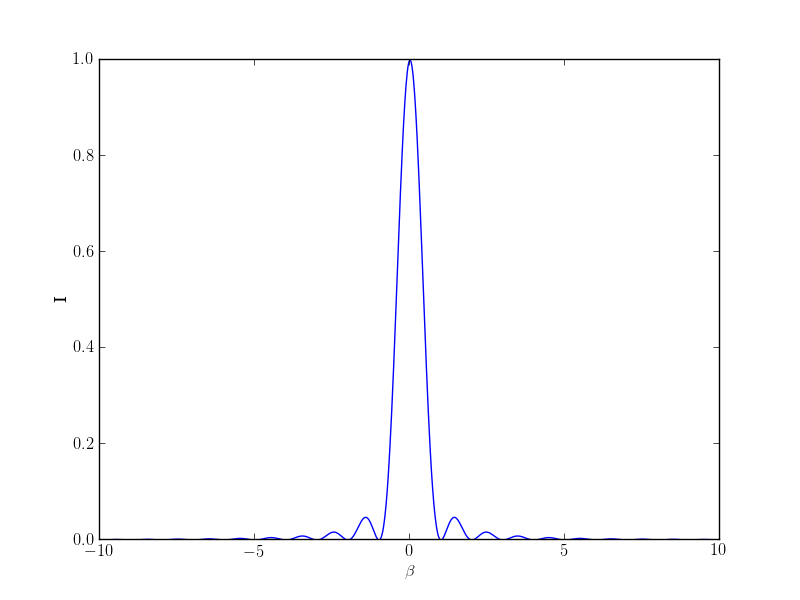
\includegraphics[scale =0.4]{fringes}
% \caption{Irradiance}
% \end{figure}
